\termin{19.04.2016}

\mdf{Definition}
In einem rechtwinkligen Dreieck
\begin{center}
\begin{tikzpicture}[font=\sffamily,scale=1.5]
\coordinate (A) at (0,0);
\coordinate (B) at (4,0);
\coordinate (C) at (4,2);

\pic["$\alpha$", draw=red, thick, -, angle eccentricity=0.7, angle radius=2cm] {angle=B--A--C};
\pic["$\cdot$", draw=red, thick, -, angle eccentricity=0.5, angle radius=0.5cm] {angle=C--B--A};

\draw [-] (A) -- (B) -- (C) -- (A);
\node [right] at (4,1) {$a$};
\node [above] at (2,1) {$b$};
\node [below] at (2,0) {$c$};
\end{tikzpicture}
\end{center}

heißt $b$ \begr{Hypotenuse}, $c$ \begr{Ankathete} zu $\alpha$ und $a$ \begr{Gegenkathete} zu $\alpha$.

Das Verhältnis $\frac{c}{b}$ heißt \begr{Kosinus} von $a$:
\begin{align*}
    \text{cos}(\alpha) &= \frac{\text{Länge der Ankathete}}{\text{Länge der Gegenkathete}}
\end{align*}

Offenbar macht diese Definition vom Kosinus nur Sinn für Winkel $0^{\circ} \leq \alpha \leq 90^{\circ}$.
\begin{center}
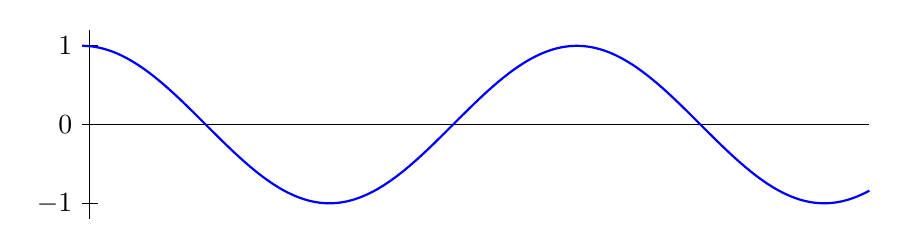
\begin{tikzpicture}[font=\sffamily]
\coordinate (A) at (0,0);
\coordinate (B) at (10,0);
\coordinate (C) at (0.1,1.2);
\coordinate (D) at (0.1,-1.2);

\draw [-] (A) -- (B);
\draw [-] (C) -- (D);

\node [left] at (0,0) {$0$};
\draw (0.2,1) -- (0,1) node[left] {$1$};
\draw (0.2,-1) -- (0,-1) node[left] {$-1$};

\draw [blue,thick] plot[variable=\x,domain=0:10,smooth,samples=200] (\x,{cos(\x r)});
\end{tikzpicture}
\end{center}

\mdf{Definition}
Seien $x = \begin{pmatrix}x_1\\\vdots\\x_n\end{pmatrix},\quad y = \begin{pmatrix}y_1\\\vdots\\y_n\end{pmatrix}$ Vektoren aus $\mathbb{R}^n$.

Das \begr{Skalarprodukt} $\langle x, y\rangle$ von $x$ und $y$ ist definiert durch
\begin{align*}
    \langle x, y\rangle &= x_1y_1 + x_2y_2 + \dots + x_ny_n
\end{align*}

Zwei Vektoren $x, y \in \mathbb{R}^n$ heißen \begr[Orthogonal (Vektoren)]{orthogonal} oder \begr[Senkrecht (Vektoren)]{senkrecht} zueinander, falls $\langle x, y\rangle = 0$.

\mdf{Definition}
Die \begr{Norm} eines Vektors $x \in \mathbb{R}^n$ ist definiert durch $\norm{x} := \sqrt{\langle x, x\rangle}$.

\mdf{Definition}
Der Winkel $\varphi$ (Phi) zwischen den Vektoren $x, y \in \mathbb{R}^n$ mit $x\neq 0, y\neq 0$ ist festgelegt durch
\begin{align*}
    \text{cos}(\varphi) &= \frac{\langle x, y\rangle}{\norm{x}\cdot\norm{y}}
\end{align*}

\begin{center}
\begin{tikzpicture}[font=\sffamily]
\draw [->] (0,0) -- (-1,1);
\draw [->,thick,red] (0,0) -- (2,3);
\draw [->] (0,0) -- (1,1.5);

\node [below left] at (-0.5,0.5) {$x$};
\node [below right] at (0.5,0.75) {$y$};
\node [below right,red] at (1.5,2.5) {$y_1 = \lambda y$};
\end{tikzpicture}
\end{center}
Die Vektoren müssen normiert werden, weil der Winkel sich sonst durch verschieden lange Vektoren verändern würde.

\mdf{Beispiel}
Im $\mathbb{R}^2$: $v_1 = \begin{pmatrix}1\\0\end{pmatrix},\quad v_2 = \begin{pmatrix}x\\y\end{pmatrix}$ mit $x, y \geq 0$.

\begin{center}
\begin{tikzpicture}[>=triangle 45,font=\sffamily,scale=1.5,decoration=brace]
\coordinate (A) at (0,0);
\coordinate (B) at (1,0);
\coordinate (C) at (2.5,2.2);

\pic["$\varphi$", draw=red, thick, -, angle eccentricity=0.7, angle radius=1.2cm] {angle=B--A--C};
	
\draw[->] (-0.5,0) -- (3.5,0) node[anchor=north west] {$x$};
\draw[->] (0,-0.5) -- (0,3.5) node[anchor=south east] {$y$};
\foreach \x in {1,2,3}
	\draw (\x cm,4pt) -- (\x cm,-4pt) node[anchor=north] {$\x$};
\foreach \y in {1,2,3}
	\draw (4pt,\y cm) -- (-4pt,\y cm) node[anchor=east] {$\y$};

\draw [thick,->] (0,0) -- (B);
\node [below] at (0.5,0) {$v_1$};

\draw [thick,->] (0,0) -- (C);
\node [above left] at (1.25,1.1) {$v_2$};

\draw [decorate, yshift=0.3cm] (0,2) -- node[above] {$x$} (2.5,2);
\draw [dashed] (0,2.2) -- (2.5,2.2);

\draw [rotate=-90, decorate, yshift=0.3cm] (-2.2,2.3) -- node[right] {$y$} (0,2.3);
\draw [dashed] (2.5,0) -- (2.5,2.2);
\end{tikzpicture}
\end{center}

Nach Definition 13:
\begin{align*}
	\text{cos}(\varphi) &= \frac{x}{\sqrt{x^2 + y^2}}
\end{align*}

Mit Skalarprodukt nach Definition 16:
\begin{align*}
	\frac{\left\langle \begin{pmatrix}1\\0\end{pmatrix}, \begin{pmatrix}x\\y\end{pmatrix} \right\rangle}{\norm{\begin{pmatrix}1\\0\end{pmatrix}}\cdot \norm{\begin{pmatrix}x\\y\end{pmatrix}}} &= \frac{1x + 0y}{\sqrt{1^2 + 0^2}\cdot\sqrt{x^2 + y^2}} = \frac{x}{\sqrt{x^2 + y^2}} = \text{cos}(\varphi)
\end{align*}

\mdf{Definition}
Eine Menge von Vektoren $v_1,\dots,v_k \in \mathbb{R}^n$ heißt \begr[Orthogonales System]{orthogonales System}, falls für alle $1\leq i, j \leq k, i\neq j$ gilt: $\langle v_i, v_j\rangle = 0$.

Ein orthogonales System $v_1,\dots,v_n \in \mathbb{R}^n$, das zusätzlich Basis von $\mathbb{R}^n$ ist und für alle $1\leq i\leq n \norm{v_i} = 1$ erfüllt, heißt \begr{Orthonormalbasis} von $\mathbb{R}^n$.

\begin{center}
\begin{tikzpicture}[>=triangle 45,font=\sffamily,scale=0.8]
\coordinate (v1) at ({2*cos(1.1 r)},{2*sin(1.1 r)});
\coordinate (v2) at ({2*cos((1.1-pi/2) r)},{2*sin((1.1-pi/2) r)});
\coordinate (c) at (0,0);

\pic["$\cdot$", draw=red, thick, -, angle eccentricity=0.6, angle radius=1.2cm] {angle=v2--c--v1};

\draw [step=2cm,gray,very thin] (-2.5,-2.5) grid (2.5,2.5);
\draw [->] (-3,0) -- (3,0) node[anchor=north west] {$x$};
\draw [->] (0,-2.5) -- (0,3) node[anchor=south east] {$y$};

\draw (0,0) circle (2);

\draw [->] (0,0) -- (v1);
\draw [->] (0,0) -- (v2);

\node [below] at (0,-2.5) {Einheitskreis};
\end{tikzpicture}\begin{tikzpicture}[>=triangle 45,font=\sffamily,scale=0.8]
\coordinate (v1) at ({2*cos(0.55 r)},{2*sin(0.55 r)});
\coordinate (v2) at ({2*cos((0.55-pi/2) r)},{2*sin((0.55-pi/2) r)});
\coordinate (c) at (0,0);

\pic["$\cdot$", draw=red, thick, -, angle eccentricity=0.6, angle radius=1.2cm] {angle=v2--c--v1};

\draw [step=2cm,gray,very thin] (-2.5,-2.5) grid (2.5,2.5);
\draw [->] (-3,0) -- (3,0) node[anchor=north west] {$x$};
\draw [->] (0,-2.5) -- (0,3) node[anchor=south east] {$y$};

\draw (0,0) circle (2);

\draw [->] (0,0) -- (v1);
\draw [->] (0,0) -- (v2);

\node [below] at (0,-2.5) {Einheitskreis};
\end{tikzpicture}\begin{tikzpicture}[>=triangle 45,font=\sffamily,scale=0.8]
\coordinate (v1) at ({2*cos(4.4 r)},{2*sin(4.4 r)});
\coordinate (v2) at ({2*cos((4.4-pi/2) r)},{2*sin((4.4-pi/2) r)});
\coordinate (c) at (0,0);

\pic["$\cdot$", draw=red, thick, -, angle eccentricity=0.6, angle radius=1.2cm] {angle=v2--c--v1};

\draw [step=2cm,gray,very thin] (-2.5,-2.5) grid (2.5,2.5);
\draw [->] (-3,0) -- (3,0) node[anchor=north west] {$x$};
\draw [->] (0,-2.5) -- (0,3) node[anchor=south east] {$y$};

\draw (0,0) circle (2);

\draw [->] (0,0) -- (v1);
\draw [->] (0,0) -- (v2);

\node [below] at (0,-2.5) {Einheitskreis};
\end{tikzpicture}
\end{center}
Das sind auch Basen.

\mdf{Satz}
\begin{enumerate}[i)]
  \item{Sei $v \in \mathbb{R}^n$. Dann gilt: $\norm{v} = 0 \Leftrightarrow v = 0$}
  \item{Für alle Vektoren $v, w \in \mathbb{R}^n$ gilt: $\langle v, w\rangle = \langle w, v\rangle$ (\glqq{}symmetrisch\grqq{})}
  \item{$\forall x, y, z \in \mathbb{R}^n$ gilt: $\langle x+y, z\rangle = \langle x, z\rangle + \langle y, z\rangle$}
  \item{$\forall x, y \in \mathbb{R}^n,\enspace \lambda, \mu \in \mathbb{R}$ gilt: $\langle\lambda x, \mu y\rangle = \lambda\mu\langle x, y\rangle$}
  \item{Ist $v_1,\dots,v_k$ ein orthogonales System und alle $v_i \neq 0$, dann sind $v_1,\dots,v_k$ linear unabhängig.}
\end{enumerate}

\textbf{Zu i)}
\begin{align*}
	\norm{v} = \sqrt{\langle v, v\rangle} = \sqrt{v_1^2+v_2^2+\dots +v_n^2} = 0 &\Leftrightarrow v_1^2+v_2^2+\dots +v_n^2 = 0 \\
	&\Leftrightarrow v_1 = v_2 = \dots = v_n = 0 \\
	&\Leftrightarrow v = 0
\end{align*}

\textbf{Zu ii)}
\begin{align*}
	\langle v, w\rangle &= v_1w_1+v_2w_2+\dots +v_nw_n\quad|\text{ Kommutativgesetz} \\
	&= w_1v_1+w_2v_2+\dots +w_nv_n = \langle w, v\rangle
\end{align*}

\textbf{Zu iii) und iv): Siehe Übung H8}

\textbf{Zu v)}
Zu zeigen: $\lambda_1v_1+\lambda_2v_2+\dots +\lambda_kv_k = 0 \Rightarrow \lambda_1 = \lambda_2 = \dots = \lambda_k = 0$

Sei also $\lambda_1v_1+\lambda_2v_2+\dots +\lambda_kv_k = 0$. Bilde das Skalarprodukt
\begin{align*}
	\langle 0, v_1\rangle &= 0 = \langle \lambda_1v_1+\dots +\lambda_kv_k, v_1\rangle \\
	\text{Nach iii)}\quad &= \langle \lambda_1v_1, v_1\rangle +\langle \lambda_2v_2, v_1\rangle+\dots +\langle \lambda_kv_k, v_1\rangle \\
	\text{Nach iv)}\quad &=\lambda_1\langle v_1, v_1\rangle + \lambda_2\langle v_2, v_1\rangle + \dots + \lambda_k\langle v_k, v_1\rangle = \lambda_1\langle v_1, v_1\rangle \\
	&= \lambda_1 \langle v_1, v_1\rangle = \lambda_1 \norm{v_1}^2\quad\text{Da } v_1\neq 0 \Rightarrow \lambda_1 = 0
\end{align*}

Analog für $i=2,\dots,k$.
\begin{align*}
	0 = \langle 0, v_i\rangle &= \langle \lambda_1v_1 + \dots + \lambda_kv_k, v_i\rangle \\
	&= \lambda_1 \langle v_1, v_i\rangle + \dots + \lambda_k \langle v_k, v_i\rangle \\
	&= \lambda_i \langle v_i, v_i\rangle\quad\text{(Da $v_1,\dots,v_k$ orth. System)} \\
	&= \lambda_i \norm{v_i}^2\quad\text{Da }v_i\neq 0\text{, folgt }\lambda_i = 0\text{.}
\end{align*}
Also $\lambda_1 = \lambda_2 = \dots = \lambda_k = 0$. Damit sind $v_1,\dots,v_k$ unabhängig.
